%
% $RCSfile: web_client_and_server.tex,v $
%
% Copyright (C) 2002-2008. Christian Heller.
%
% Permission is granted to copy, distribute and/or modify this document
% under the terms of the GNU Free Documentation License, Version 1.1 or
% any later version published by the Free Software Foundation; with no
% Invariant Sections, with no Front-Cover Texts and with no Back-Cover
% Texts. A copy of the license is included in the section entitled
% "GNU Free Documentation License".
%
% http://www.cybop.net
% - Cybernetics Oriented Programming -
%
% http://www.resmedicinae.org
% - Information in Medicine -
%
% Version: $Revision: 1.1 $ $Date: 2008-08-19 20:41:09 $ $Author: christian $
% Authors: Christian Heller <christian.heller@tuxtax.de>
%

\section{Web Client and Server}
\label{web_client_and_server_heading}
\index{Web Client and Server}
\index{Internet}
\index{Web Server}
\index{Web Client}
\index{Web Browser}
\index{Applets}
\index{Servlets}
\index{Transfer Control Protocol}
\index{TCP}
\index{Internet Protocol}
\index{IP}
\index{Hypertext Transfer Protocol}
\index{HTTP}

With the emerge of the \emph{Internet}, several new kinds of services like
\emph{Email}, \emph{File Transfer}, \emph{Web} etc. became popular. The web
service allows information to be published in form of a \emph{Web Page}. Web
pages can be written in markup formats like \emph{Hypertext Markup Language}
(HTML) and \emph{Extensible Markup Language} (XML) or, using special tags, as
\emph{Java Server Pages-} (JSP) and \emph{PHP Hypertext Preprocessor-} (PHP)
instructions. Before being displayed, the latter two need to be translated by a
preprocessor inside the web server, into HTML.

\begin{figure}[ht]
    \begin{center}
        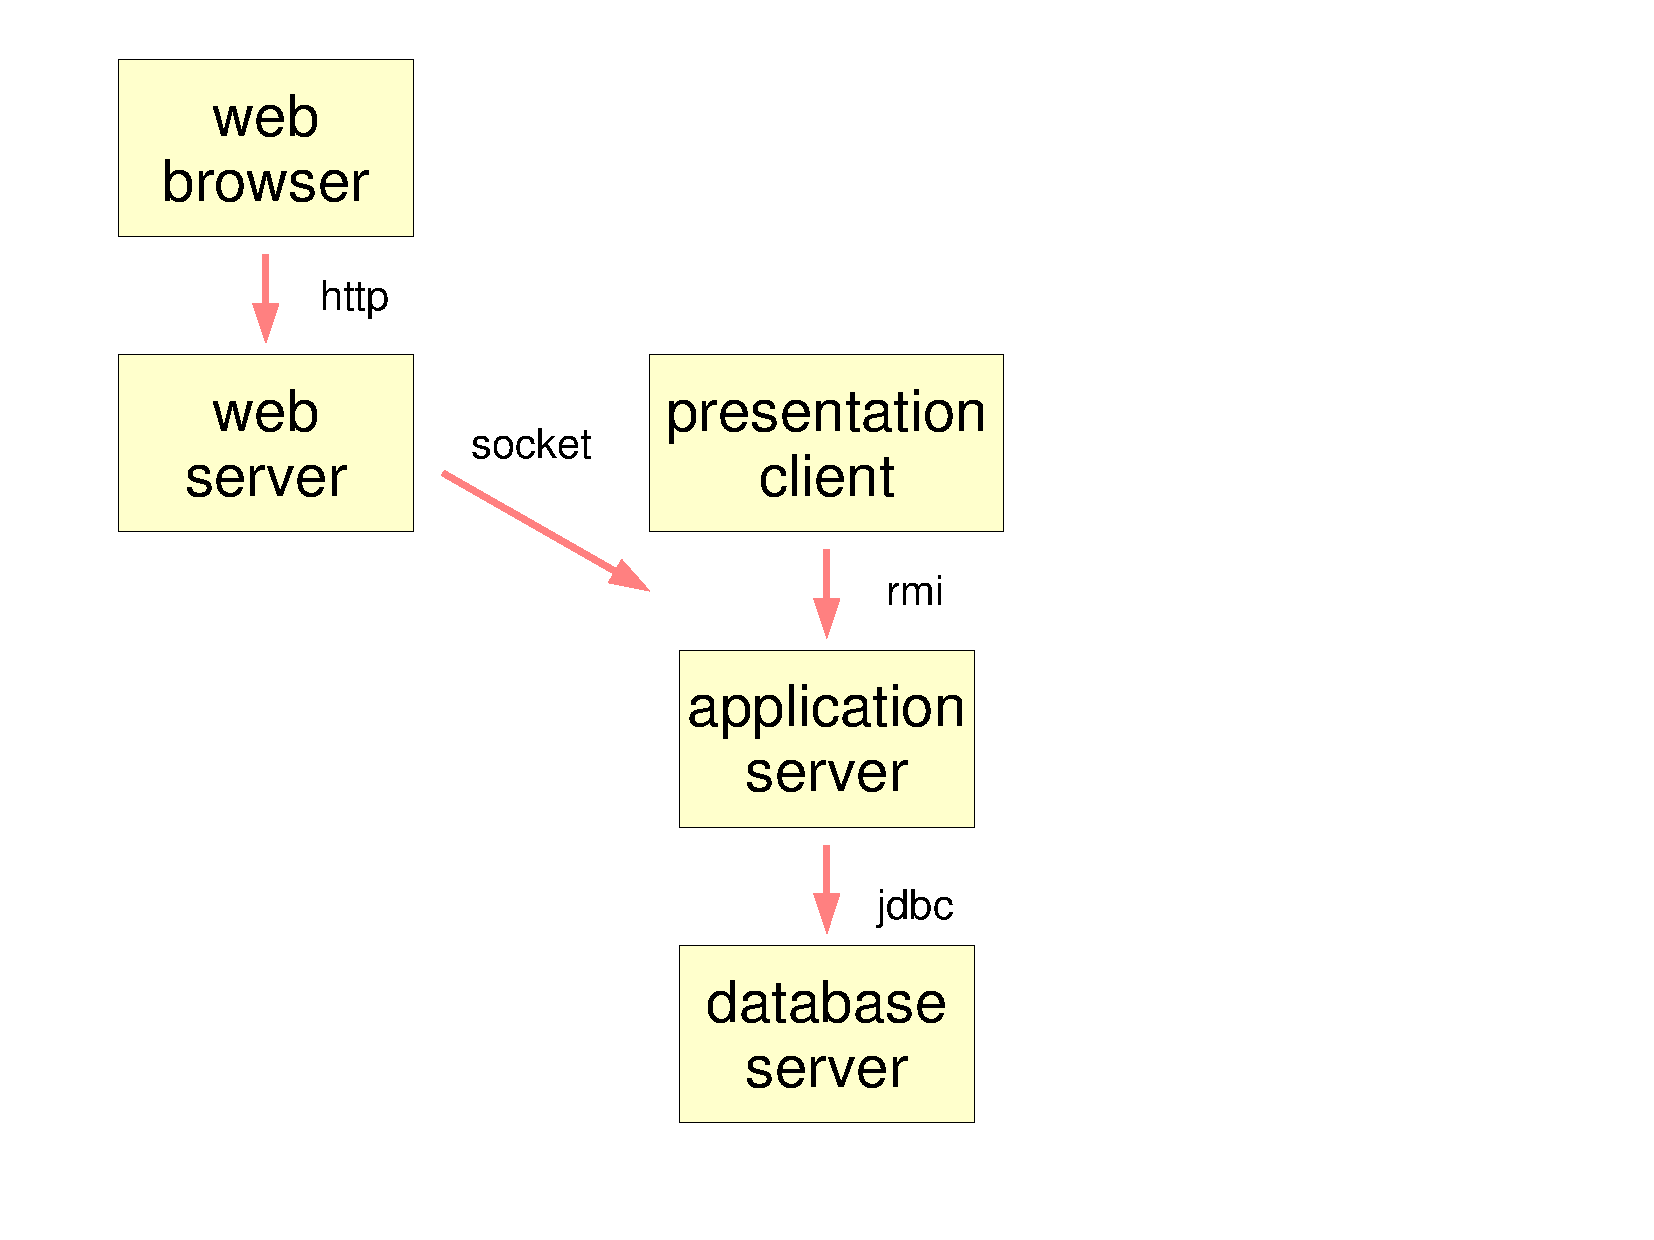
\includegraphics[scale=0.3,angle=-90]{graphic/web.pdf}
        \caption{Web Client and Server}
        \label{web_figure}
    \end{center}
\end{figure}

The principle as shown in figure \ref{web_figure} is easy: A \emph{Web Server}
stores web pages which can be accessed by clients called \emph{Web Browser}.
Browsers extract and translate (render) the (graphical) information given in
form of a web page and display them. But they are also able to handle actions
such as keyboard input or mouse click, and send these information back to the
web server.

Moreover, browsers can locally execute small programs called \emph{Applets}
which were downloaded from the web server. Their counterpart are \emph{Servlets}
which are executed in multiple threads on the web server, offering the actual
services.

Web communication is based on standards like the \emph{Transfer Control Protocol}/
\emph{Internet Protocol} (TCP/IP) and the \emph{Hypertext Transfer Protocol}
(HTTP) \cite{tanenbaum2000}. Section \ref{systems_interconnection_heading} will
systematise them together with other standards for system interconnection. The
socket mechanism may be used to connect a web server to an application server.

Many other aspects are important when talking about internet services. There is
the issue of security, there is performance, user-friendliness and many more
which will not be discussed further here, since it would exceed the frame of
this work.
